\documentclass[11pt,onside]{article}
\usepackage[a4paper]{geometry}
\usepackage[utf8]{inputenc}
\usepackage[english]{babel}
\usepackage{lipsum}
\usepackage{bm}
\usepackage{upgreek}
\usepackage[noend]{algpseudocode}
\usepackage{algorithm}
\usepackage{amsmath}
\usepackage{float}
\usepackage{graphicx} % Required for including images

% mathtools for: Aboxed (put box on last equation in align envirenment)
\usepackage{microtype} %improves the spacing between words and letters

%% COLOR DEFINITIONS

\usepackage[svgnames]{xcolor} % Enabling mixing colors and color's call by 'svgnames'

\definecolor{MyColor1}{rgb}{0.2,0.4,0.6} %mix personal color
\newcommand{\textb}{\color{Black} \usefont{OT1}{lmss}{m}{n}}
\newcommand{\blue}{\color{MyColor1} \usefont{OT1}{lmss}{m}{n}}
\newcommand{\blueb}{\color{MyColor1} \usefont{OT1}{lmss}{b}{n}}
\newcommand{\red}{\color{LightCoral} \usefont{OT1}{lmss}{m}{n}}
\newcommand{\green}{\color{Turquoise} \usefont{OT1}{lmss}{m}{n}}

\DeclareMathOperator{\trace}{trace}
\DeclareMathOperator{\diag}{diag}

%% FONTS AND COLORS

%    SECTIONS

\usepackage{titlesec}
\usepackage{sectsty}
%%%%%%%%%%%%%%%%%%%%%%%%
%set section/subsections HEADINGS font and color
\sectionfont{\color{MyColor1}}  % sets colour of sections
\subsectionfont{\color{MyColor1}}  % sets colour of sections

%set section enumerator to arabic number (see footnotes markings alternatives)
\renewcommand\thesection{\arabic{section}.} %define sections numbering
\renewcommand\thesubsection{\thesection\arabic{subsection}} %subsec.num.

%define new section style
\newcommand{\mysection}{
\titleformat{\section} [runin] {\usefont{OT1}{lmss}{b}{n}\color{MyColor1}} 
{\thesection} {3pt} {} } 


%	CAPTIONS
\usepackage{caption}
\usepackage{subcaption}
%%%%%%%%%%%%%%%%%%%%%%%%
\captionsetup[figure]{labelfont={color=Turquoise}}


%		!!!EQUATION (ARRAY) --> USING ALIGN INSTEAD
%using amsmath package to redefine eq. numeration (1.1, 1.2, ...) 
\renewcommand{\theequation}{\thesection\arabic{equation}}



\makeatletter
\let\reftagform@=\tagform@
\def\tagform@#1{\maketag@@@{(\ignorespaces\textcolor{red}{#1}\unskip\@@italiccorr)}}
\renewcommand{\eqref}[1]{\textup{\reftagform@{\ref{#1}}}}
\makeatother
\usepackage{hyperref}
\hypersetup{colorlinks=true}

% For labeling top of page on every page but first one:
\usepackage{fancyhdr}

% PREPARE TITLE:
\title{\blue Adversarial Robustness-toolbox \\
\blueb Generate Counter Examples}
\author{Fast Gradient Method, Basic Iterative Method, Deep Fool}

\renewcommand{\rmdefault}{phv} % Arial Font
\renewcommand{\sfdefault}{phv} % Arial Font

\pagestyle{fancy}
\fancyhead{}
\fancyhead[CO,CE]{{\small{{\bf{Adversarial Robustness-toolbox}} - Counter Examples}}}
 


\begin{document}
\maketitle
\section{Train Simple CNN Model}

\begin{algorithm}[H]
\caption{MNIST Model Training and Verification}
\begin{algorithmic}
    

\State Load MNIST dataset into $(X_{\text{train}}, Y_{\text{train}})$, $(X_{\text{test}}, Y_{\text{test}})$
\State Preprocess:
\State $X_{\text{train}} \gets \text{reshape}(X_{\text{train}}, 60000, 28, 28, 1) / 255$
\State $X_{\text{test}} \gets \text{reshape}(X_{\text{test}}, 10000, 28, 28, 1) / 255$
\State $Y_{\text{train\_cat}} \gets \text{to\_categorical}(Y_{\text{train}}, 10)$
\State $Y_{\text{test\_cat}} \gets \text{to\_categorical}(Y_{\text{test}}, 10)$
\State Define $M$ as Sequential with layers:
\State $M.\text{add}(\text{Conv2D}(32, (3, 3), \text{activation}='relu', \text{input\_shape}=(28, 28, 1)))$
\State $M.\text{add}(\text{MaxPooling2D}((2, 2)))$
\State $M.\text{add}(\text{Flatten}())$
\State $M.\text{add}(\text{Dense}(128, \text{activation}='relu'))$
\State $M.\text{add}(\text{Dense}(10, \text{activation}='softmax'))$
\State Compile $M$ with loss='categorical\_crossentropy', optimizer='adam', metrics=['accuracy']
\State Train $M$ on $(X_{\text{train}}, Y_{\text{train\_cat}})$ for 10 epochs, batch size 200
\State Save $M$ to 'mnist\_model.h5'
\State $P \gets M.\text{predict}(X_{\text{test}})$ \Comment{P for predictions}
\State $L_{\text{pred}} \gets \text{argmax}(P, \text{axis}=1)$ \Comment{L\_pred for predicted labels}
\State Extract and save correct predictions:
\State $ \text{correct\_indices} \gets \{i | L_{\text{pred}}[i] = Y_{\text{test}}[i]\}$
\State $E_{\text{correct}} \gets X_{\text{test}}[\text{correct\_indices}]$
\State $L_{\text{correct}} \gets Y_{\text{test}}[\text{correct\_indices}]$
\State $\text{save}(E_{\text{correct}}, 'correct\_examples.npy')$
\State $\text{save}(L_{\text{correct}}, 'correct\_labels.npy')$

\end{algorithmic}
\end{algorithm}

\section{FSGM without target variables}
\begin{algorithm}[H]
\caption{Generating and Analyzing Adversarial Examples}
\begin{algorithmic}[1]
\Require Trained CNN model $M$, saved correct examples $E_{\text{correct}}.npy$, labels $L_{\text{correct}}.npy$
\Ensure Adversarial examples $X_{\text{adv}}$, confusion matrix $CM$
\State Initialize TensorFlow and disable eager execution
\State $M \gets \text{load\_model}('mnist\_model.h5')$
\State $E_{\text{correct}} \gets \text{load}('correct\_examples.npy') / 255$
\State $L_{\text{correct}} \gets \text{load}('correct\_labels.npy')$
\State Classifier $\gets$ KerasClassifier(model=$M$, clip\_values=$(0, 1)$)
\State Attack $\gets$ FastGradientMethod(Classifier, eps=$0.1$)
\State $X_{\text{adv}} \gets$ Attack.generate($E_{\text{correct}}$)
\State $Y_{\text{adv}} \gets \text{argmax}(\text{Classifier.predict}(X_{\text{adv}}), \text{axis}=1)$
\State $CM \gets \text{confusion\_matrix}(L_{\text{correct}}, Y_{\text{adv}}, \text{labels}=\text{range}(10))$
\State Visualize $CM$ with heatmap, axis labels 'Predicted Label' and 'True Label', and title 'Confusion Matrix'
\end{algorithmic}
\end{algorithm}


\begin{figure*}[h]
\centering
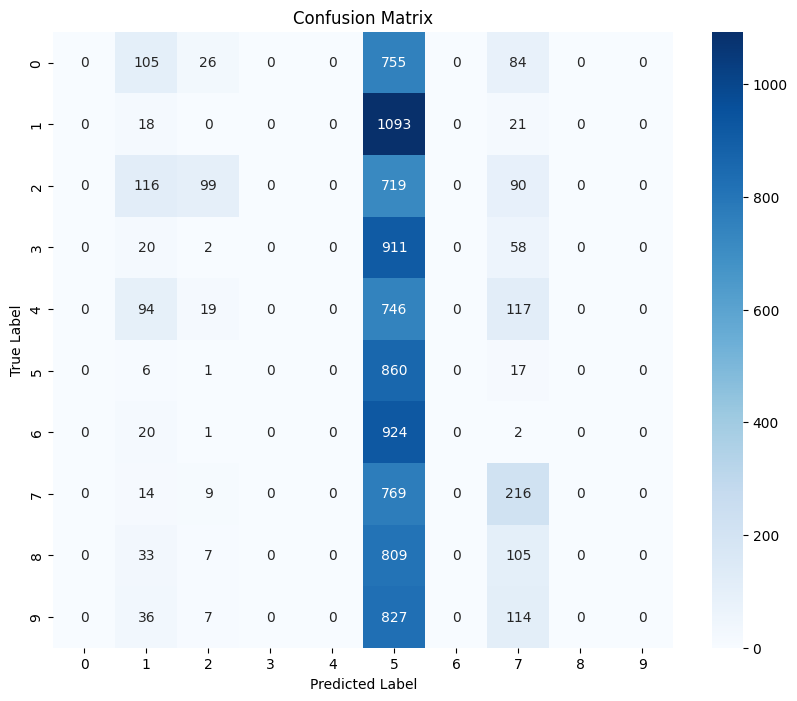
\includegraphics[width=0.8\textwidth]{V1_images/FGM_without_target.png}
\caption{CM FSGM without target variables}
\label{fig: FSGM without target variables}
\end{figure*}


\section{FSGM with target variables}

\begin{algorithm}[H]

\caption{Adversarial Example Generation and Confusion Matrix Computation}
\begin{algorithmic}[1]
\State Attack $\gets$ FastGradientMethod(Classifier, eps=0.1)
\State $X_{\text{adv}} \gets$ Attack.generate($x=$ correct\_examples, $y=$ correct\_labels)
\State $Y_{\text{adv}} \gets \text{argmax}(\text{Classifier.predict}(X_{\text{adv}}), \text{axis}=1)$
\State $CM \gets \text{confusion\_matrix}(\text{correct\_labels}, Y_{\text{adv}}, \text{labels}=\text{range}(10))$
\State Visualize $CM$ as a heatmap
\end{algorithmic}
\end{algorithm}

\begin{figure*}[h]
\centering
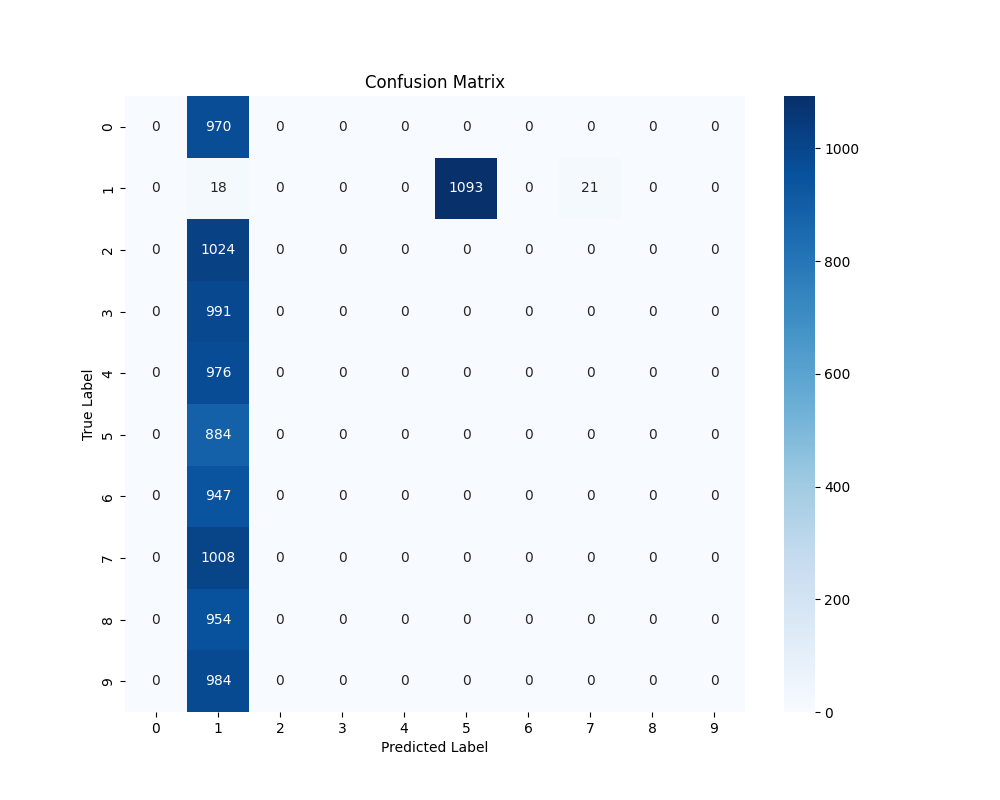
\includegraphics[width=1\textwidth]{V1_images/FGM_with_target.png}
\caption{CM FSGM with target variables}
\label{fig: FSGM with target variables}
\end{figure*}


\section{FSGM without target variables (Multiple Examples Generation)}

\begin{algorithm}[H]
\caption{Repeated Adversarial Example Generation and Aggregated Confusion Matrix}
\begin{algorithmic}[1]
\State $num\_attacks \gets 5$
\State $sum\_cm \gets \text{zero matrix of size } 10 \times 10$
\For{$i \gets 1$ \textbf{to} $num\_attacks$}
    \State $x\_adv \gets \text{attack.generate}(x=\text{correct\_examples})$
    \State $y\_adv \gets \text{argmax}(\text{classifier.predict}(x\_adv), \text{axis}=1)$
    \State $cm \gets \text{confusion\_matrix}(\text{correct\_labels}, y\_adv, \text{labels}=\text{range}(10))$
    \State $sum\_cm \gets sum\_cm + cm$
\EndFor
\State Visualize $sum\_cm$ as a heatmap
\end{algorithmic}
\end{algorithm}

\begin{figure*}[h]
\centering
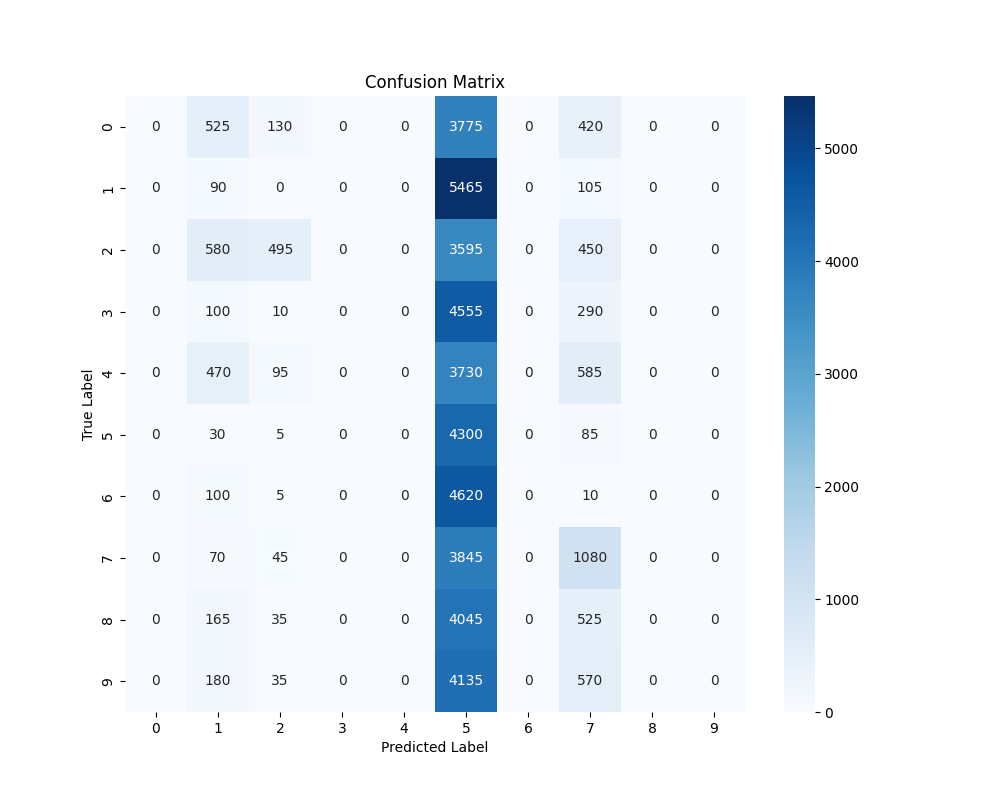
\includegraphics[width=1\textwidth]{V1_images/mul_attacks_FGM_without_target.png}
\caption{CM FSGM without target variables (Multiple Examples Generation)}
\label{fig:FSGM without target variables (Multiple Examples Generation)}
\end{figure*}



\section{FSGM with target variables (Multiple Examples Generation)}
\begin{algorithm}[H]
\caption{Repeated Adversarial Example Generation and Aggregated Confusion Matrix}
\begin{algorithmic}[1]
\State $num\_attacks \gets 5$
\State $sum\_cm \gets \text{zero matrix of size } 10 \times 10$
\For{$i \gets 1$ \textbf{to} $num\_attacks$}
    \State $x\_adv \gets \text{attack.generate}(x=\text{correct\_examples}, y=\text{correct\_labels})$
    \State $y\_adv \gets \text{argmax}(\text{classifier.predict}(x\_adv), \text{axis}=1)$
    \State $cm \gets \text{confusion\_matrix}(\text{correct\_labels}, y\_adv, \text{labels}=\text{range}(10))$
    \State $sum\_cm \gets sum\_cm + cm$
\EndFor
\State Visualize $sum\_cm$ as a heatmap
\end{algorithmic}
\end{algorithm}

\begin{figure*}[h]
\centering
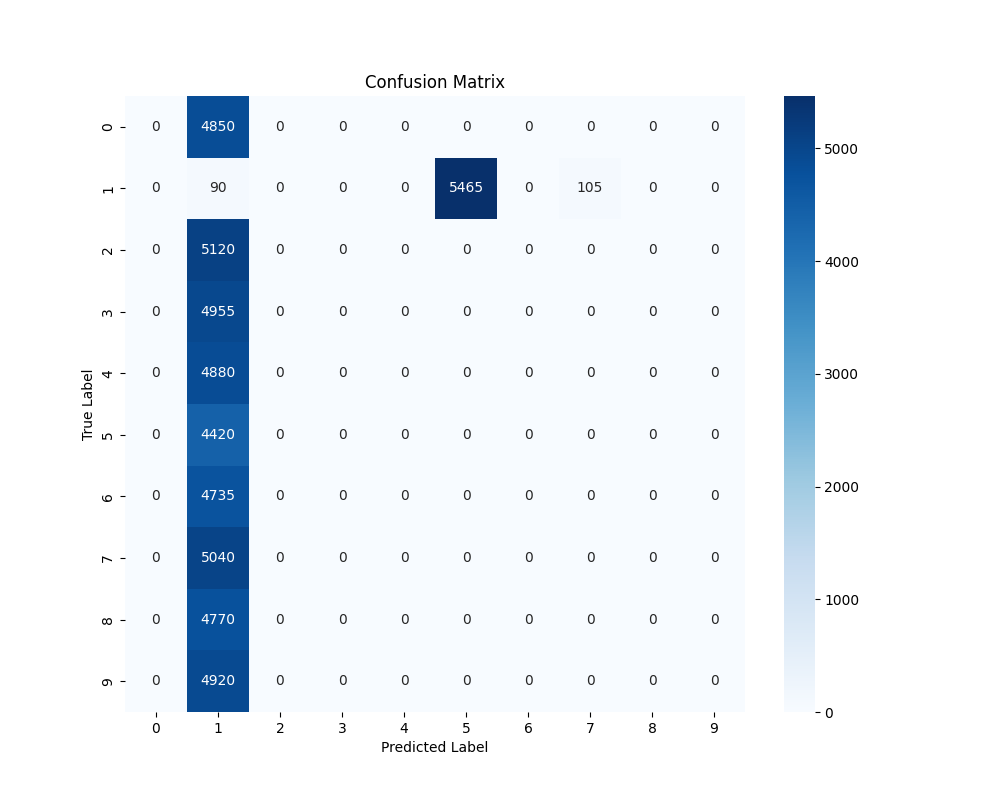
\includegraphics[width=1\textwidth]{V1_images/mul_attacks_FGM_with_target.png}
\caption{CM FSGM without target variables (Multiple Examples Generation)}
\label{fig:FSGM with target variables (Multiple Examples Generation)}
\end{figure*}



\section{BIM without target variables}


\begin{algorithm}[H]
\caption{Adversarial Example Generation with Basic Iterative Method and Confusion Matrix Computation}
\begin{algorithmic}[1]
\State Import BasicIterativeMethod from art.attacks.evasion
\State Attack $\gets$ BasicIterativeMethod(Classifier, eps=0.1, max\_iter=10)
\State $X_{\text{adv}} \gets$ Attack.generate($x=$ correct\_examples)
\State $Y_{\text{adv}} \gets \text{argmax}(\text{Classifier.predict}(X_{\text{adv}}), \text{axis}=1)$
\State $CM \gets \text{confusion\_matrix}(\text{correct\_labels}, Y_{\text{adv}}, \text{labels}=\text{range}(10))$
\State Visualize $CM$ as a heatmap
\end{algorithmic}
\end{algorithm}


\begin{figure*}[h]
\centering
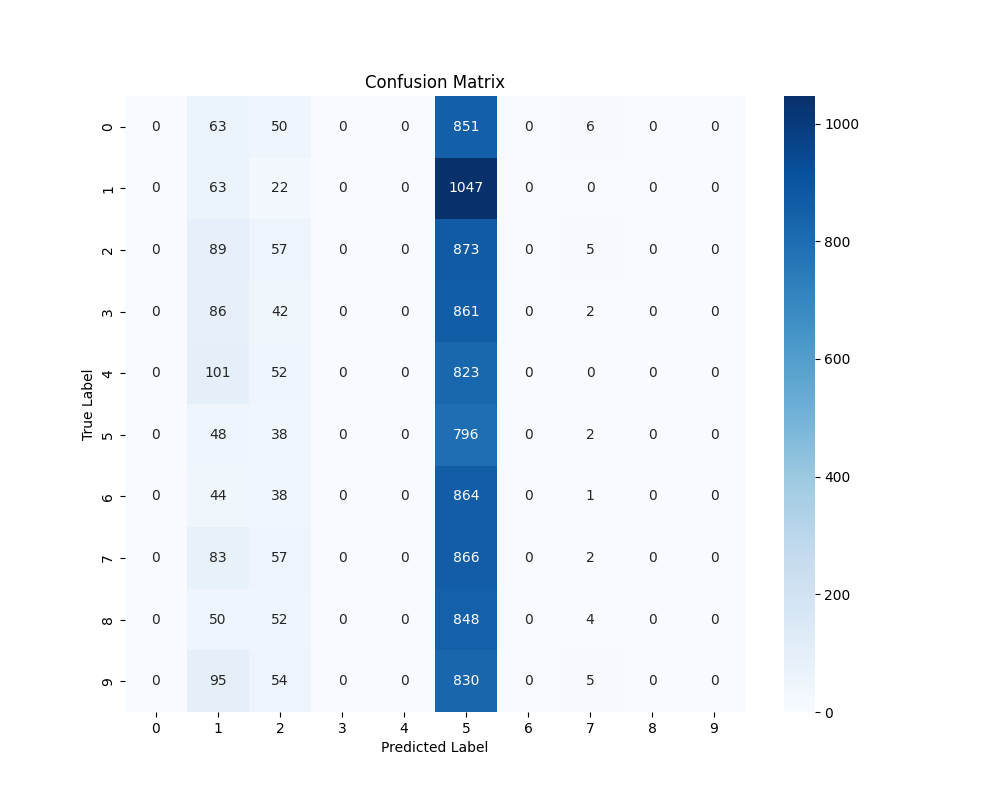
\includegraphics[width=1\textwidth]{V1_images/BIK_without_target.png}
\caption{CM BIM without target variables)}
\label{fig: BIM without target variables)}
\end{figure*}


\section{BIM with target variables}

\begin{algorithm}[H]
\caption{Adversarial Example Generation with Basic Iterative Method and Confusion Matrix Computation}
\begin{algorithmic}[1]
\State Import BasicIterativeMethod from art.attacks.evasion
\State Attack $\gets$ BasicIterativeMethod(Classifier, eps=0.1, max\_iter=10)
\State $X_{\text{adv}} \gets$ Attack.generate($x=$ correct\_examples,y=\text{correct\_labels})
\State $Y_{\text{adv}} \gets \text{argmax}(\text{Classifier.predict}(X_{\text{adv}}), \text{axis}=1)$
\State $CM \gets \text{confusion\_matrix}(\text{correct\_labels}, Y_{\text{adv}}, \text{labels}=\text{range}(10))$
\State Visualize $CM$ as a heatmap
\end{algorithmic}
\end{algorithm}

\begin{figure*}[h]
\centering
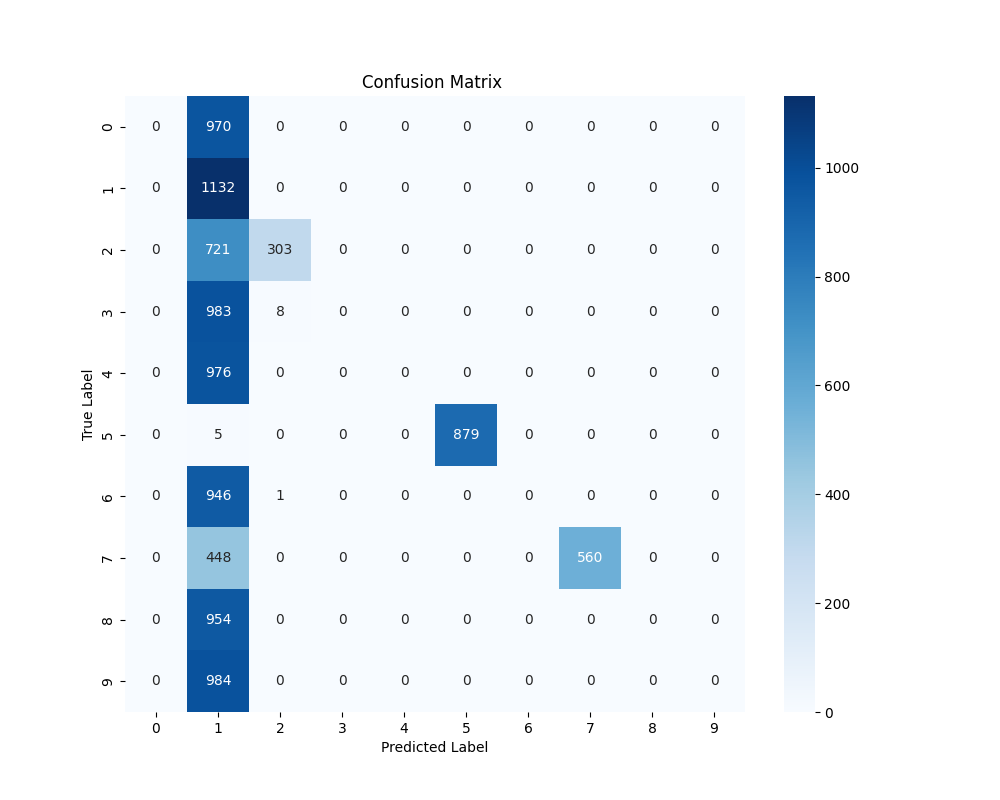
\includegraphics[width=1\textwidth]{V1_images/BIM_with_target.png}
\caption{BIM with target variables)}
\label{fig: BIM with target variables)}
\end{figure*}


\section{BIM without target variables (Multiple Examples Generation)}


\begin{algorithm}[H]
\caption{Repeated Adversarial Example Generation and Aggregated Confusion Matrix}
\begin{algorithmic}[1]
\State $num\_attacks \gets 5$
\State $sum\_cm \gets \text{zero matrix of size } 10 \times 10$
\For{$i \gets 1$ \textbf{to} $num\_attacks$}
    \State $x\_adv \gets \text{attack.generate}(x=\text{correct\_examples})$
    \State $y\_adv \gets \text{argmax}(\text{classifier.predict}(x\_adv), \text{axis}=1)$
    \State $cm \gets \text{confusion\_matrix}(\text{correct\_labels}, y\_adv, \text{labels}=\text{range}(10))$
    \State $sum\_cm \gets sum\_cm + cm$
\EndFor
\State Visualize $sum\_cm$ as a heatmap
\end{algorithmic}
\end{algorithm}

\begin{figure*}[h]
\centering
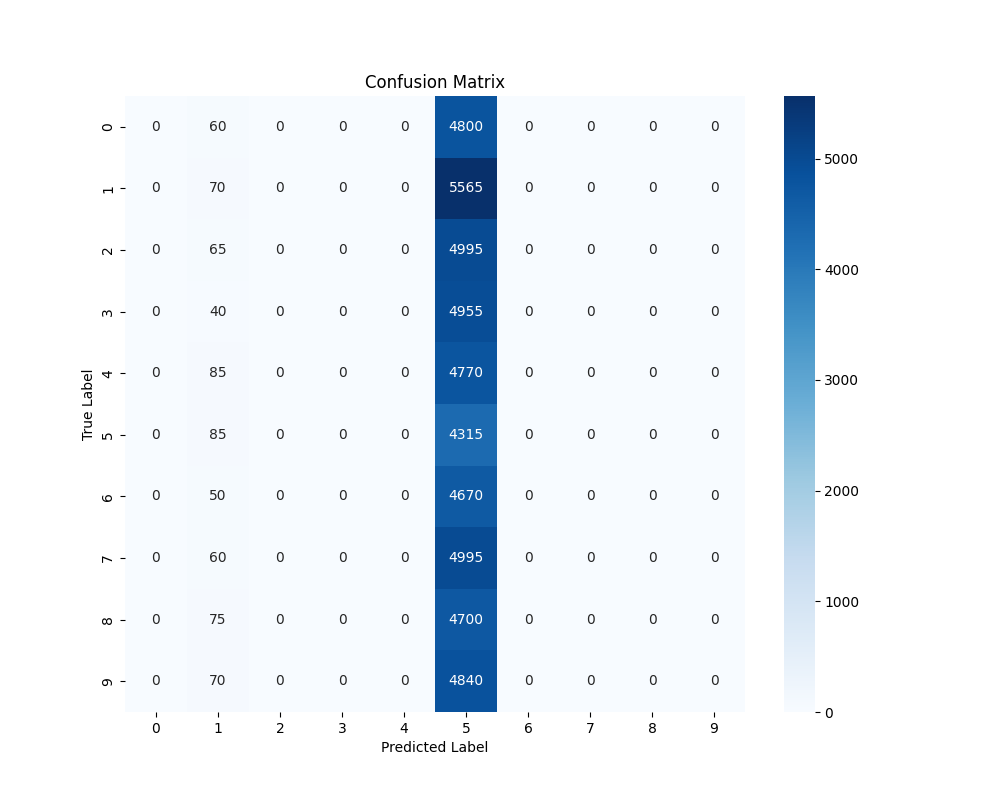
\includegraphics[width=1\textwidth]{V1_images/mul_BIM_without_target.png}
\caption{BIM without target variables (Multiple Examples Generation)}
\label{fig: BIM without target variables (Multiple Examples Generation)}
\end{figure*}

\section{BIM with target variables (Multiple Examples Generation)}

\begin{algorithm}[H]
\caption{Repeated Adversarial Example Generation and Aggregated Confusion Matrix}
\begin{algorithmic}[1]
\State $num\_attacks \gets 5$
\State $sum\_cm \gets \text{zero matrix of size } 10 \times 10$
\For{$i \gets 1$ \textbf{to} $num\_attacks$}
    \State $x\_adv \gets \text{attack.generate}(x=\text{correct\_examples},y=\text{correct\_labels})$
    \State $y\_adv \gets \text{argmax}(\text{classifier.predict}(x\_adv), \text{axis}=1)$
    \State $cm \gets \text{confusion\_matrix}(\text{correct\_labels}, y\_adv, \text{labels}=\text{range}(10))$
    \State $sum\_cm \gets sum\_cm + cm$
\EndFor
\State Visualize $sum\_cm$ as a heatmap
\end{algorithmic}
\end{algorithm}

\begin{figure*}[h]
\centering
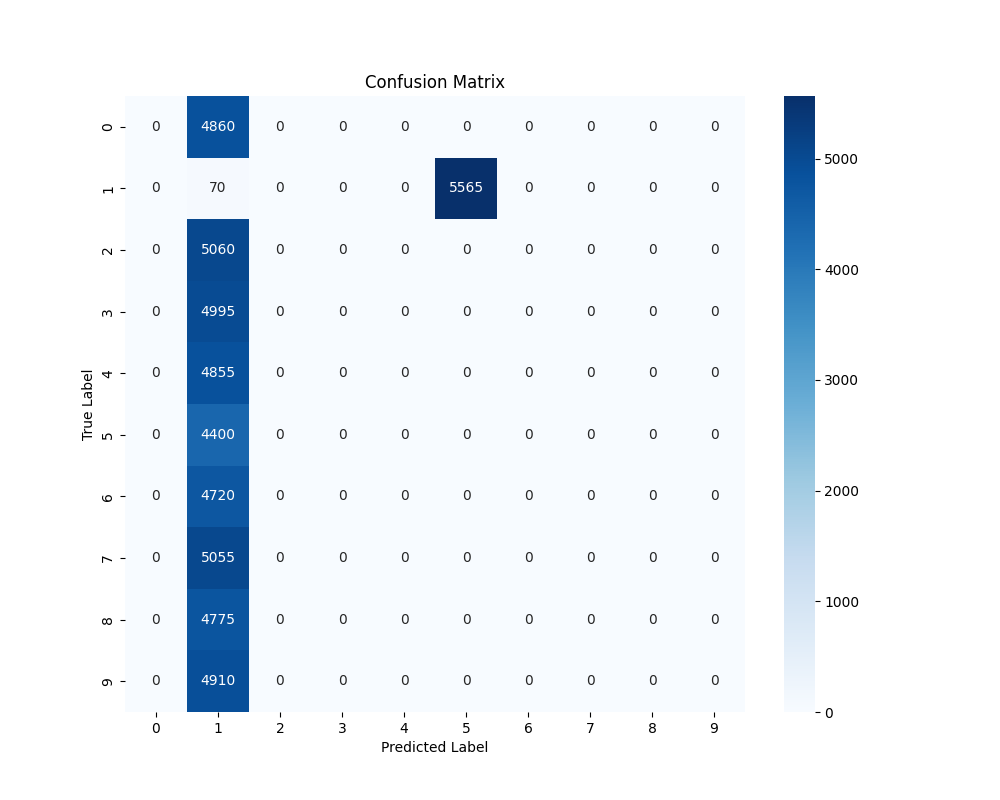
\includegraphics[width=1\textwidth]{V1_images/mul_BIM_with_target.png}
\caption{BIM without target variables (Multiple Examples Generation)}
\label{fig: BIM without target variables (Multiple Examples Generation)}
\end{figure*}


\section{DeepFool without target variables}

\begin{algorithm}[H]
\caption{Adversarial Example Generation with DeepFool and Confusion Matrix Computation}
\begin{algorithmic}[1]
\State Import DeepFool from art.attacks.evasion
\State Attack $\gets$ DeepFool(Classifier)
\State $X_{\text{adv}} \gets$ Attack.generate($x=$ correct\_examples)
\State $Y_{\text{adv}} \gets \text{argmax}(\text{Classifier.predict}(X_{\text{adv}}), \text{axis}=1)$
\State $CM \gets \text{confusion\_matrix}(\text{correct\_labels}, Y_{\text{adv}}, \text{labels}=\text{range}(10))$
\State Visualize $CM$ as a heatmap
\end{algorithmic}
\end{algorithm}

\begin{figure*}[h]
\centering
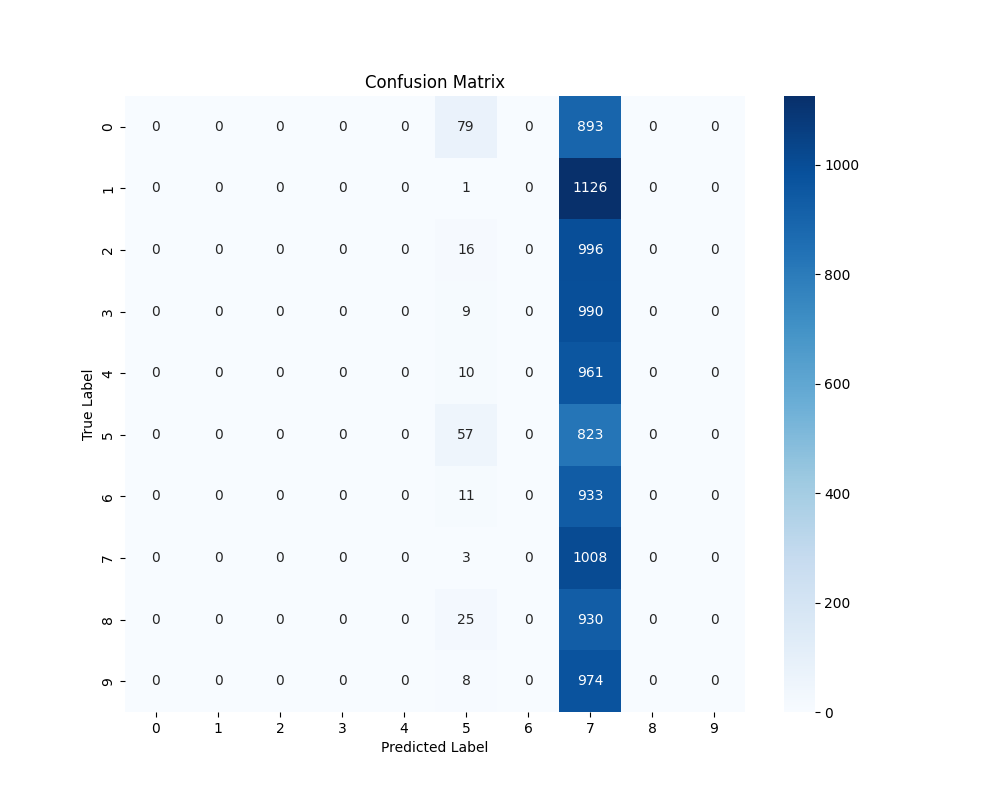
\includegraphics[width=1\textwidth]{V1_images/DeepFool_withOUT_target.png}
\caption{Deepfool without target variables)}
\label{fig: DeepFool without target variables}
\end{figure*}


\section{DeepFool with target variables}

\begin{algorithm}[H]
\caption{Adversarial Example Generation with DeepFool and Confusion Matrix Computation}
\begin{algorithmic}[1]
\State Import DeepFool from art.attacks.evasion
\State Attack $\gets$ DeepFool(Classifier)
\State $X_{\text{adv}} \gets$ Attack.generate($x=$ correct\_examples,y=\text{correct\_labels})
\State $Y_{\text{adv}} \gets \text{argmax}(\text{Classifier.predict}(X_{\text{adv}}), \text{axis}=1)$
\State $CM \gets \text{confusion\_matrix}(\text{correct\_labels}, Y_{\text{adv}}, \text{labels}=\text{range}(10))$
\State Visualize $CM$ as a heatmap
\end{algorithmic}
\end{algorithm}

\begin{figure*}[h]
\centering
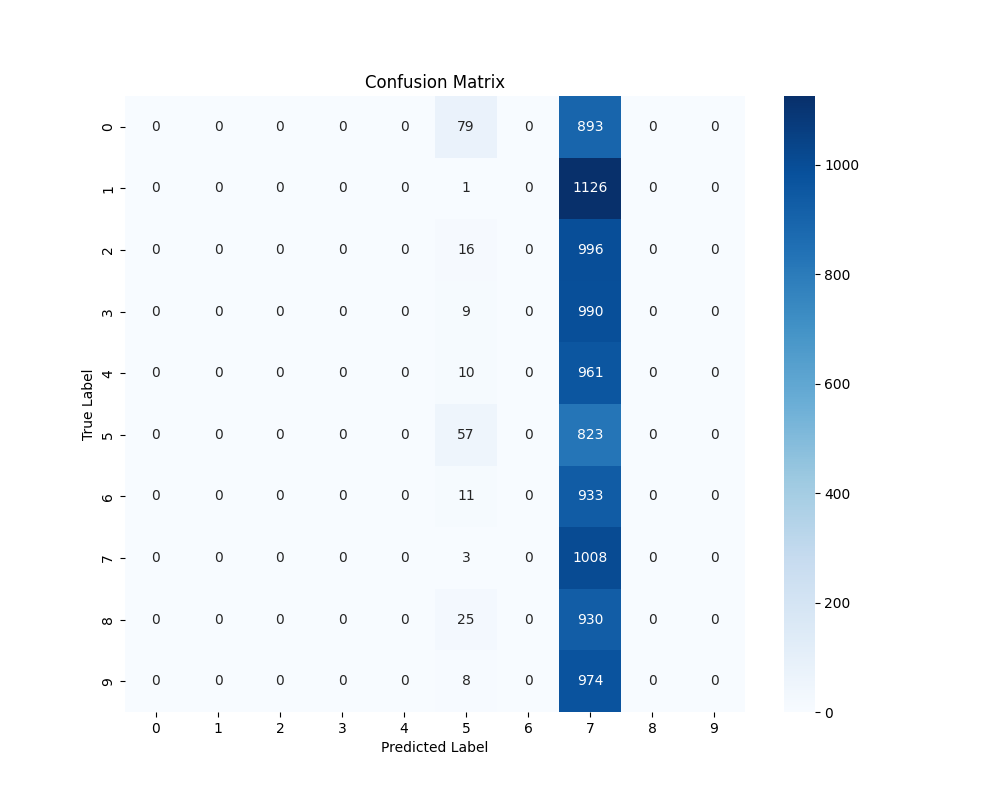
\includegraphics[width=1\textwidth]{V1_images/DeepFool_with_target.png}
\caption{DeepFool with target variables)}
\label{fig: DeepFool with target variables}
\end{figure*}



\section{DeepFool without target variables (Multiple Examples Generation)}
\begin{algorithm}[H]
\caption{Repeated Adversarial Example Generation and Aggregated Confusion Matrix}
\begin{algorithmic}[1]
\State $num\_attacks \gets 5$
\State $sum\_cm \gets \text{zero matrix of size } 10 \times 10$
\For{$i \gets 1$ \textbf{to} $num\_attacks$}
    \State $x\_adv \gets \text{attack.generate}(x=\text{correct\_examples})$
    \State $y\_adv \gets \text{argmax}(\text{classifier.predict}(x\_adv), \text{axis}=1)$
    \State $cm \gets \text{confusion\_matrix}(\text{correct\_labels}, y\_adv, \text{labels}=\text{range}(10))$
    \State $sum\_cm \gets sum\_cm + cm$
\EndFor
\State Visualize $sum\_cm$ as a heatmap
\end{algorithmic}
\end{algorithm}

\begin{figure*}[h]
\centering
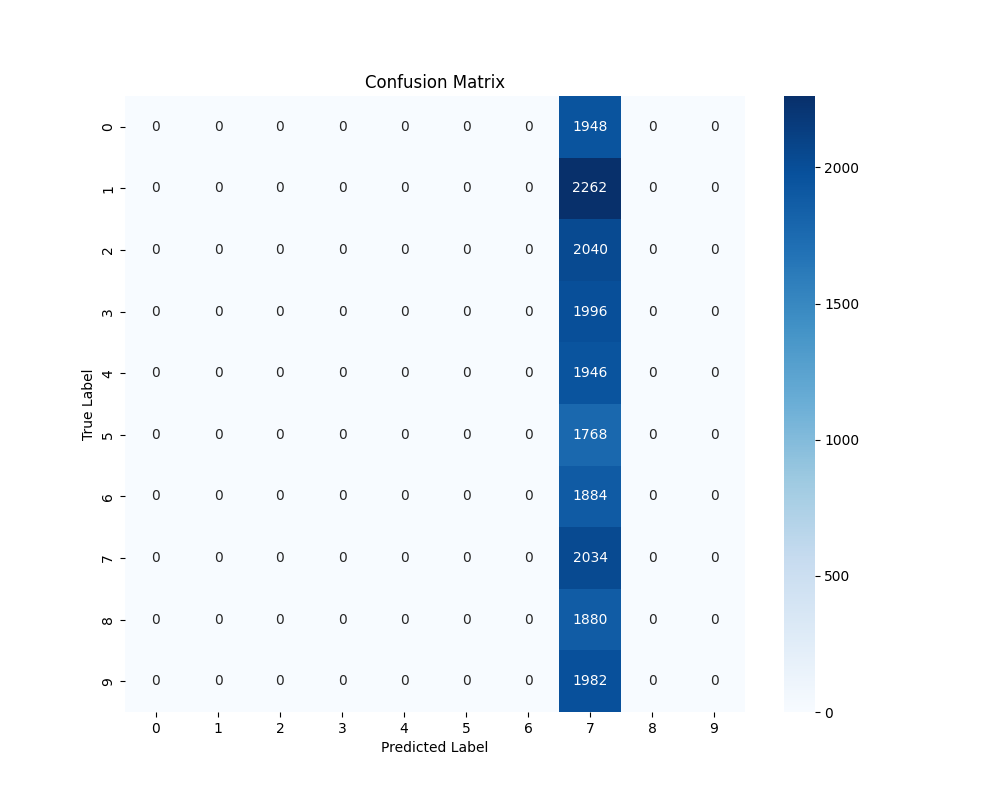
\includegraphics[width=1\textwidth]{V1_images/Mul_DeepFool_withOUT_target.png}
\caption{DeepFool without target variables (Multiple Examples Generation}
\label{fig: DeepFool without target variables (Multiple Examples Generation)}
\end{figure*}


\section{DeepFool with target variables (Multiple Examples Generation)}

\begin{algorithm}[H]
\caption{Repeated Adversarial Example Generation and Aggregated Confusion Matrix}
\begin{algorithmic}[1]
\State $num\_attacks \gets 5$
\State $sum\_cm \gets \text{zero matrix of size } 10 \times 10$
\For{$i \gets 1$ \textbf{to} $num\_attacks$}
    \State $x\_adv \gets \text{attack.generate}(x=\text{correct\_examples},y=\text{correct\_labels})$
    \State $y\_adv \gets \text{argmax}(\text{classifier.predict}(x\_adv), \text{axis}=1)$
    \State $cm \gets \text{confusion\_matrix}(\text{correct\_labels}, y\_adv, \text{labels}=\text{range}(10))$
    \State $sum\_cm \gets sum\_cm + cm$
\EndFor
\State Visualize $sum\_cm$ as a heatmap
\end{algorithmic}
\end{algorithm}


\begin{figure*}[h]
\centering
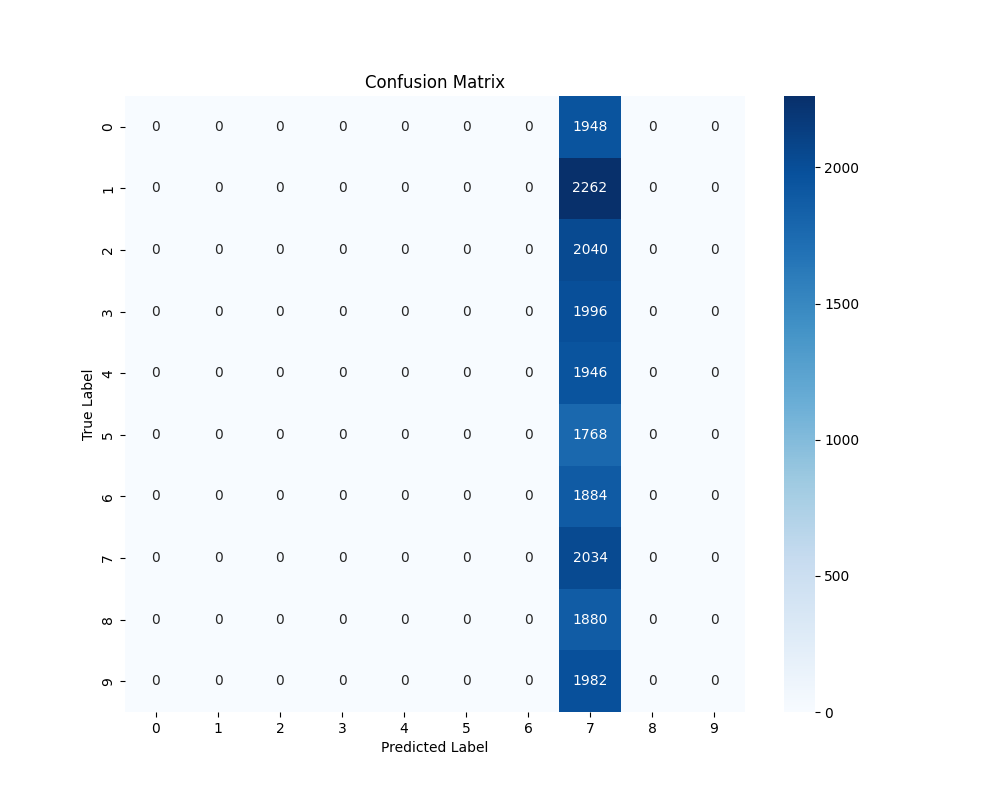
\includegraphics[width=1\textwidth]{V1_images/Mul_DeepFool_with_target.png}
\caption{DeepFool with target variables (Multiple Examples Generation)}
\label{fig: DeepFool with target variables (Multiple Examples Generation)}
\end{figure*}

\end{document}